\newpage
\section{Preventivo} \label{Preventivo}

Viene di seguito riportato il preventivo per il \NomeProgetto{}; esso si divide, per ogni periodo, in:
\begin{itemize}
	\item \textbf{Prospetto orario}: presenta la distribuzione oraria e la suddivisione nei ruoli per ogni membro del gruppo \gruppo;
	\item \textbf{Prospetto economico}: presenta le ore di impegno calcolate per i ruoli coinvolti ed il rispettivo costo.
\end{itemize}
La suddivisione oraria viene fatta tenendo conto delle seguenti regole:
\begin{itemize}
	\item Ogni membro del gruppo dovrà sostenere una mole di lavoro comparabile, quindi il totale delle ore dovrà essere equamente distribuito tra i membri;
	\item Ogni membro del gruppo dovrà ricoprire ogni ruolo almeno una volta durante il ciclo di sviluppo del prodotto;
	\item In nessun caso si dovrà verificare un conflitto di interessi in cui un \ver{} debba	controllare il proprio lavoro.
\end{itemize}
Le sigle utilizzate per i vari ruoli saranno:
\begin{itemize}
	\item \textbf{Re}: \RdP;
	\item \textbf{Ad}: \adm;
	\item \textbf{An}: \ana;
	\item \textbf{Pr}: \prog;
	\item \textbf{Pg}: \progr;
	\item \textbf{Ve}: \ver.
\end{itemize}
Per il preventivo si tiene conto che i primi due periodi sono considerati di investimento del gruppo e non a carico del committente, per cui le ore di impegno svolte durante questi non saranno conteggiate nelle ore totali da retribuire.
\newpage
\subsection{Attività di investimento del gruppo}
\subsubsection{Analisi dei requisiti}
\paragraph{Prospetto orario}
Il prospetto orario per questo periodo è illustrato in tabella.
\begin{table}[H]
	\centerline{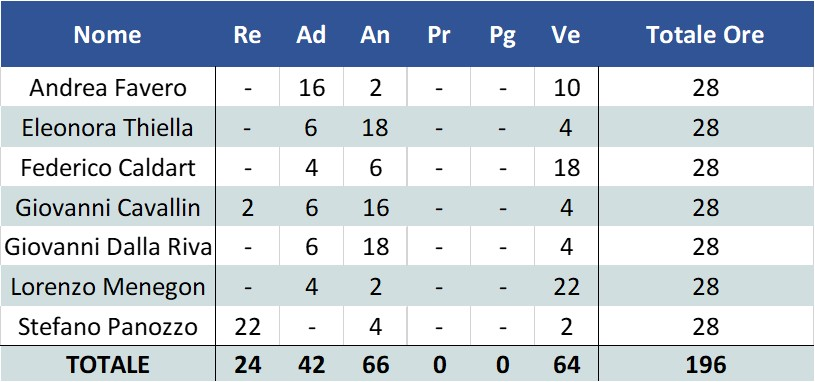
\includegraphics[scale=0.7]{img/Preventivo/AnalisiRequisitiOrario.jpg}}
	\caption{Prospetto Orario: Analisi dei requisiti}
	\clearpage
\end{table}
La raffigurazione grafica della suddivisione dei ruoli all'interno del gruppo è così rappresentata: 
\begin{figure}[H]
	\centerline{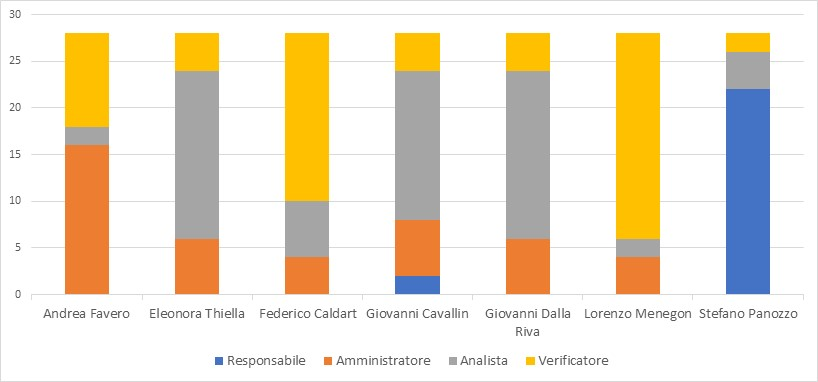
\includegraphics[scale=0.85]{img/Preventivo/Istogrammi/AnalisiRequisiti.jpg}}
	\caption{Raffigurazione Prospetto Orario: Analisi dei requisiti}
	\clearpage
\end{figure}
\newpage
\paragraph{Prospetto economico}
Il prospetto economico per questo periodo è illustrato in tabella. Notare che le spese per questa attività non sono a carico del committente.
\begin{table}[H]
	\centerline{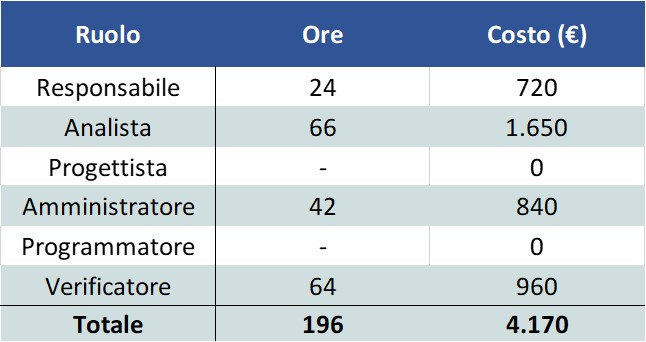
\includegraphics[scale=0.7]{img/Preventivo/AnalisiRequisitiEconomico.jpg}}
	\caption{Prospetto Economico: Analisi dei requisiti}
	\clearpage
\end{table}
La raffigurazione grafica del peso di ogni ruolo sul costo totale è così rappresentata: 
\begin{figure}[H]
	\centerline{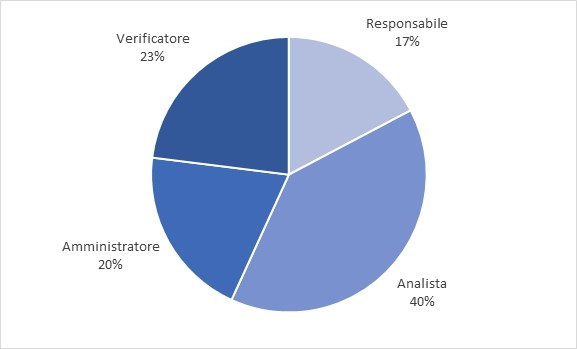
\includegraphics[scale=0.9]{img/Preventivo/Torte/AnalisiRequisiti.jpg}}
	\caption{Raffigurazione Prospetto Economico: Analisi dei requisiti}
	\clearpage
\end{figure}
\newpage
\subsubsection{Analisi dei requisiti in dettaglio}
\paragraph{Prospetto orario}
Il prospetto orario per questo periodo è illustrato in tabella.
\begin{table}[H]
	\centerline{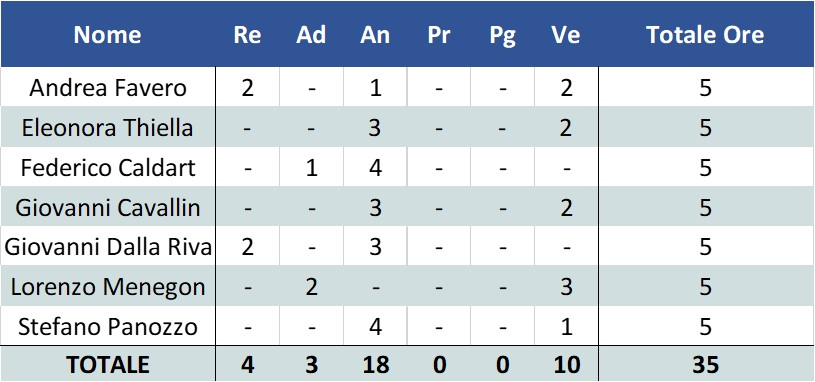
\includegraphics[scale=0.7]{img/Preventivo/AnalisiRequisitiDettaglioOrario.jpg}}
	\caption{Prospetto Orario: Analisi dei requisiti in dettaglio}
	\clearpage
\end{table}
La raffigurazione grafica della suddivisione dei ruoli all'interno del gruppo è così rappresentata: 
\begin{figure}[H]
	\centerline{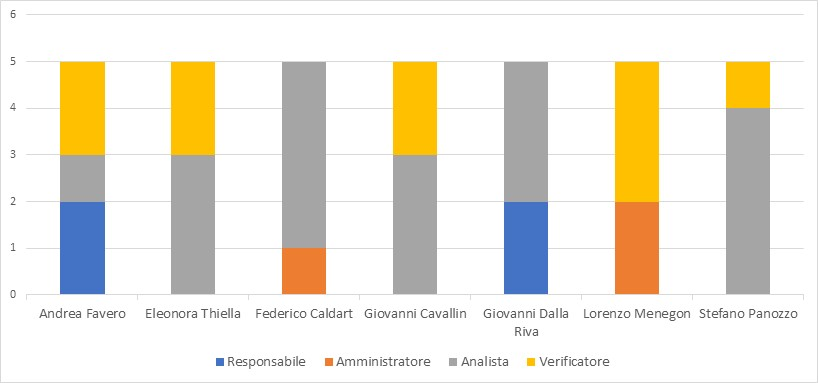
\includegraphics[scale=0.85]{img/Preventivo/Istogrammi/AnalisiRequisitiDettaglio.jpg}}
	\caption{Raffigurazione Prospetto Orario: Analisi dei requisiti in dettaglio}
	\clearpage
\end{figure}
\newpage
\paragraph{Prospetto economico} \label{PreventivoAnalisiRequisitiDettaglio}
Il prospetto economico per questo periodo è illustrato in tabella. Notare che le spese per questa attività non sono a carico del committente.
\begin{table}[H]
	\centerline{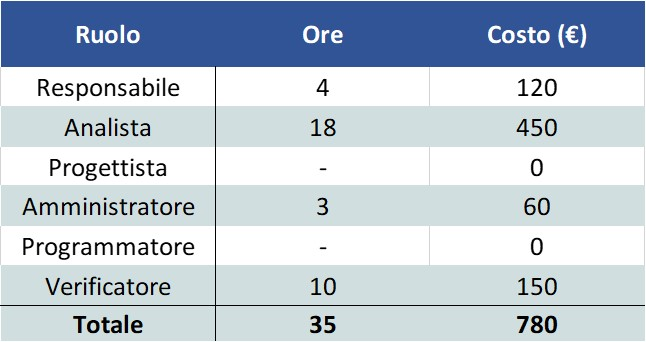
\includegraphics[scale=0.7]{img/Preventivo/AnalisiRequisitiDettaglioEconomico.jpg}}
	\caption{Prospetto Economico: Analisi dei requisiti in dettaglio}
	\clearpage
\end{table}
La raffigurazione grafica del peso di ogni ruolo sul costo totale è così rappresentata: 
\begin{figure}[H]
	\centerline{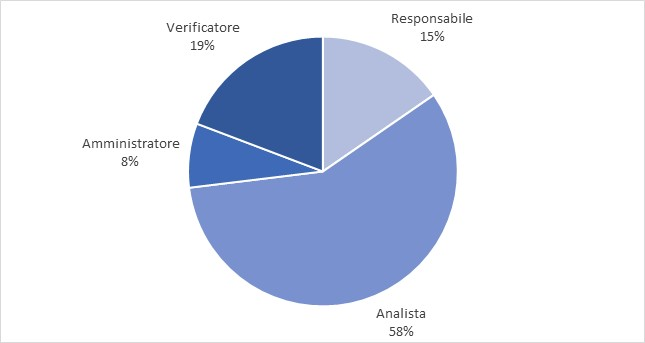
\includegraphics[scale=0.9]{img/Preventivo/Torte/AnalisiRequisitiDettaglio.jpg}}
	\caption{Raffigurazione Prospetto Economico: Analisi dei requisiti in dettaglio}
	\clearpage
\end{figure}
\newpage
\subsection{Attività a carico del committente}
\subsubsection{Prototipazione}
\paragraph{Prospetto orario}
Il prospetto orario per questo periodo è illustrato in tabella.
\begin{table}[H]
	\centerline{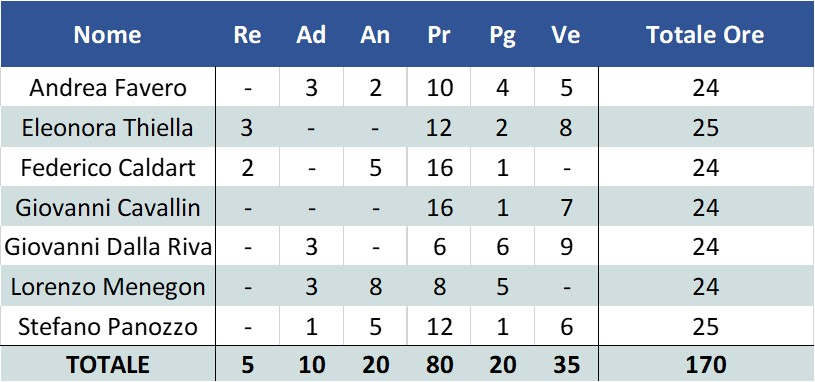
\includegraphics[scale=0.7]{img/Preventivo/PrototipazioneOrario.jpg}}
	\caption{Prospetto Orario: Prototipazione}
	\clearpage
\end{table}
La raffigurazione grafica della suddivisione dei ruoli all'interno del gruppo è così rappresentata: 
\begin{figure}[H]
	\centerline{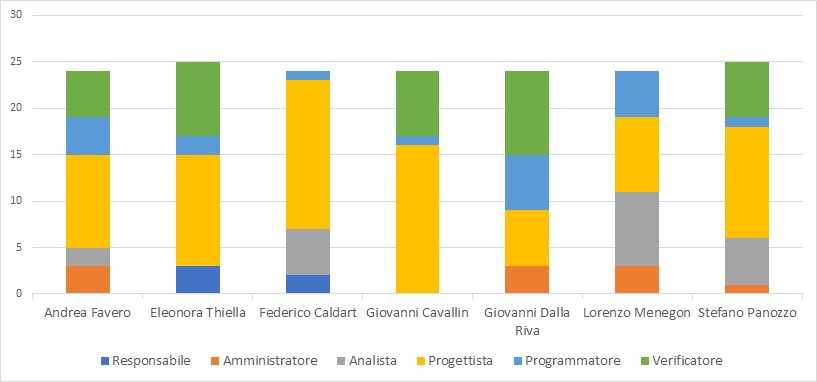
\includegraphics[scale=0.85]{img/Preventivo/Istogrammi/Prototipazione.jpg}}
	\caption{Raffigurazione Prospetto Orario: Prototipazione}
	\clearpage
\end{figure}
\newpage
\paragraph{Prospetto economico}
Il prospetto economico per questo periodo è illustrato in tabella. 
\begin{table}[H]
	\centerline{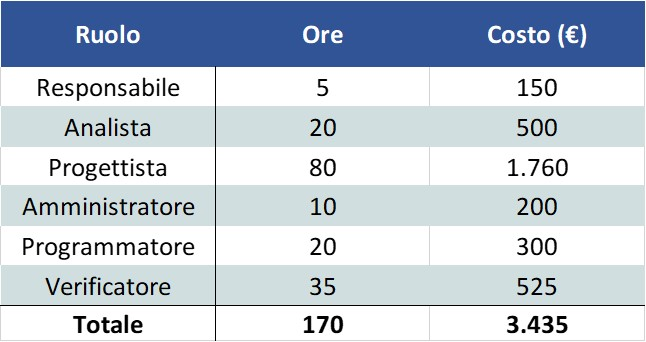
\includegraphics[scale=0.7]{img/Preventivo/PrototipazioneEconomico.jpg}}
	\caption{Prospetto Economico: Prototipazione}
	\clearpage
\end{table}
La raffigurazione grafica del peso di ogni ruolo sul costo totale è così rappresentata: 
\begin{figure}[H]
	\centerline{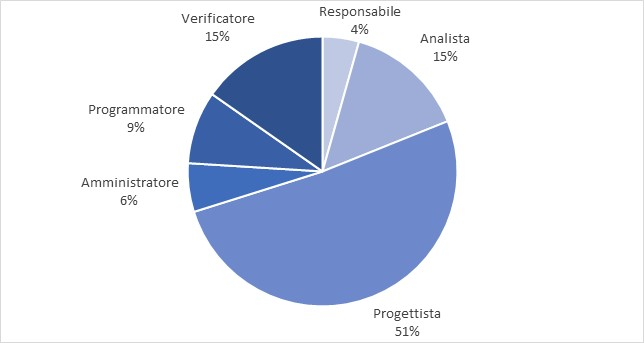
\includegraphics[scale=0.9]{img/Preventivo/Torte/Prototipazione.jpg}}
	\caption{Raffigurazione Prospetto Economico: Prototipazione}
	\clearpage
\end{figure}
\newpage
\subsubsection{Prototipazione in dettaglio}
\paragraph{Prospetto orario}
Il prospetto orario per questo periodo è illustrato in tabella.
\begin{table}[H]
	\centerline{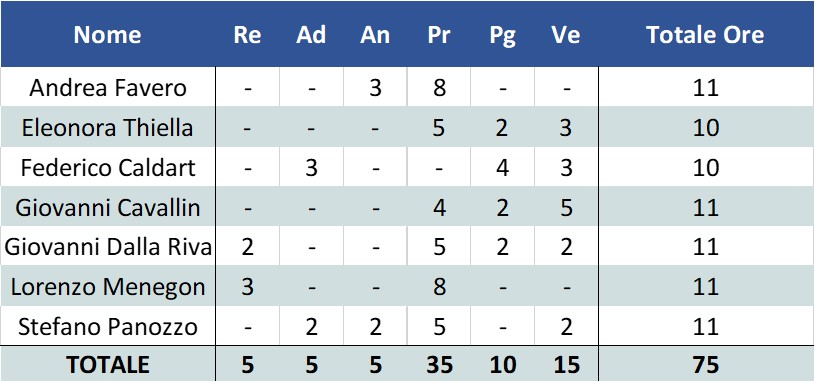
\includegraphics[scale=0.7]{img/Preventivo/PrototipazioneDettaglioOrario.jpg}}
	\caption{Prospetto Orario: Prototipazione in dettaglio}
	\clearpage
\end{table}
La raffigurazione grafica della suddivisione dei ruoli all'interno del gruppo è così rappresentata: 
\begin{figure}[H]
	\centerline{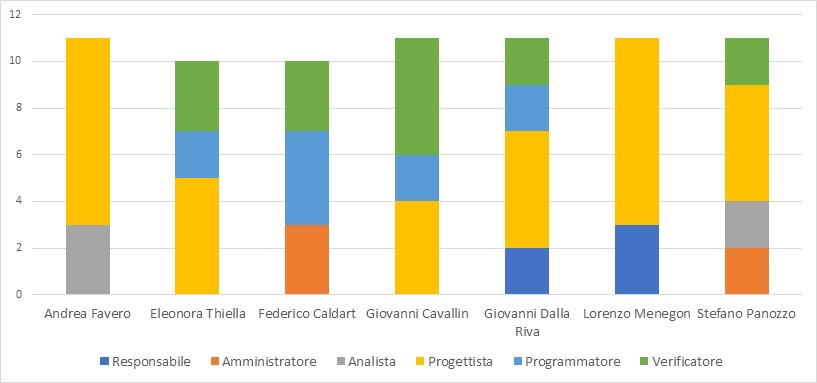
\includegraphics[scale=0.85]{img/Preventivo/Istogrammi/PrototipazioneDettaglio.jpg}}
	\caption{Raffigurazione Prospetto Orario: Prototipazione in dettaglio}
	\clearpage
\end{figure}
\newpage
\paragraph{Prospetto economico}
Il prospetto economico per questo periodo è illustrato in tabella. 
\begin{table}[H]
	\centerline{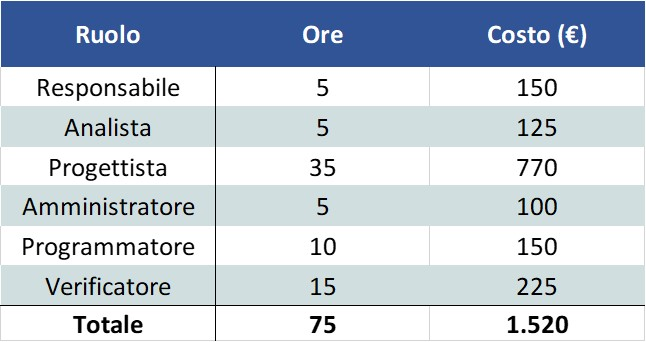
\includegraphics[scale=0.7]{img/Preventivo/PrototipazioneDettaglioEconomico.jpg}}
	\caption{Prospetto Economico: Prototipazione in dettaglio}
	\clearpage
\end{table}
La raffigurazione grafica del peso di ogni ruolo sul costo totale è così rappresentata:
\begin{figure}[H]
	\centerline{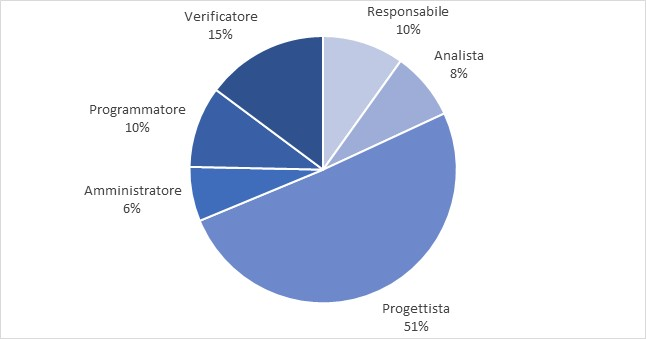
\includegraphics[scale=0.9]{img/Preventivo/Torte/PrototipazioneDettaglio.jpg}}
	\caption{Raffigurazione Prospetto Economico: Prototipazione in dettaglio}
	\clearpage
\end{figure} 
\newpage
\subsubsection{Progettazione finale e Codifica}
\paragraph{Prospetto orario}
Il prospetto orario per questo periodo è illustrato in tabella.
\begin{table}[H]
	\centerline{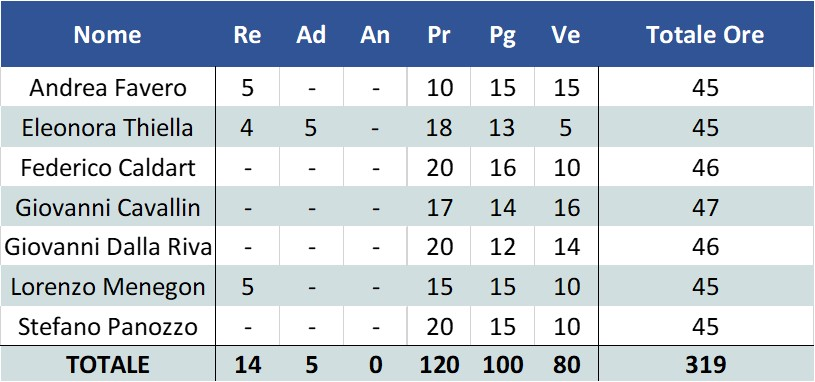
\includegraphics[scale=0.7]{img/Preventivo/ProgettazioneFinaleCodificaOrario.jpg}}
	\caption{Prospetto Orario: Progettazione finale e Codifica}
	\clearpage
\end{table}
La raffigurazione grafica della suddivisione dei ruoli all'interno del gruppo è così rappresentata: 
\begin{figure}[H]
	\centerline{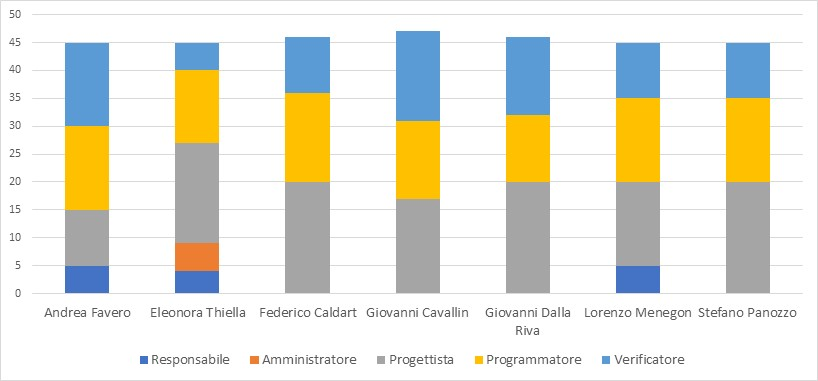
\includegraphics[scale=0.85]{img/Preventivo/Istogrammi/ProgettazioneFinaleCodifica.jpg}}
	\caption{Raffigurazione Prospetto Orario: Progettazione finale e Codifica}
	\clearpage
\end{figure}
\newpage
\paragraph{Prospetto economico}
Il prospetto economico per questo periodo è illustrato in tabella. 
\begin{table}[H]
	\centerline{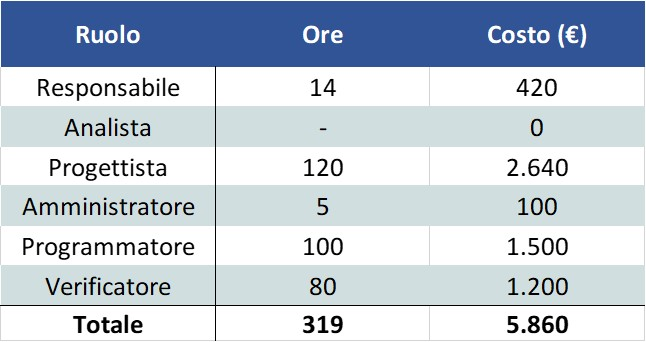
\includegraphics[scale=0.7]{img/Preventivo/ProgettazioneFinaleCodificaEconomico.jpg}}
	\caption{Prospetto Economico: Progettazione finale e Codifica}
	\clearpage
\end{table}
La raffigurazione grafica del peso di ogni ruolo sul costo totale è così rappresentata: 
\begin{figure}[H]
	\centerline{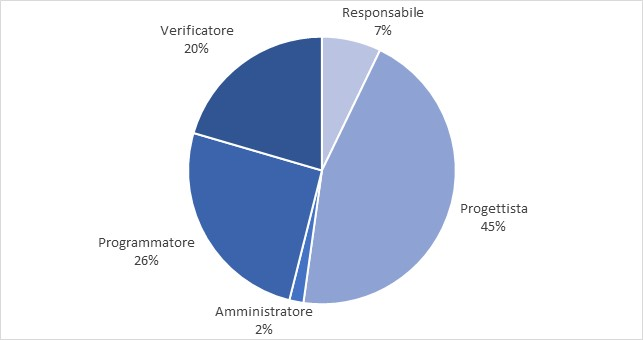
\includegraphics[scale=0.9]{img/Preventivo/Torte/ProgettazioneFinaleCodifica.jpg}}
	\caption{Raffigurazione Prospetto Economico: Progettazione finale e Codifica}
	\clearpage
\end{figure} 
\newpage
\subsubsection{Codifica in dettaglio, Validazione e Collaudo}
\paragraph{Prospetto orario}
Il prospetto orario per questo periodo è illustrato in tabella.
\begin{table}[H]
	\centerline{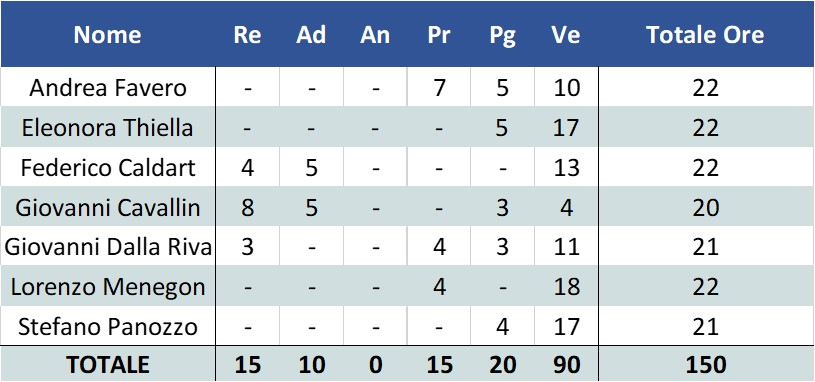
\includegraphics[scale=0.7]{img/Preventivo/CodDettaglioValidazioneCollaudoOrario.jpg}}
	\caption{Prospetto Orario: Codifica in dettaglio, Validazione e Collaudo}
	\clearpage
\end{table}
La raffigurazione grafica della suddivisione dei ruoli all'interno del gruppo è così rappresentata: 
\begin{figure}[H]
	\centerline{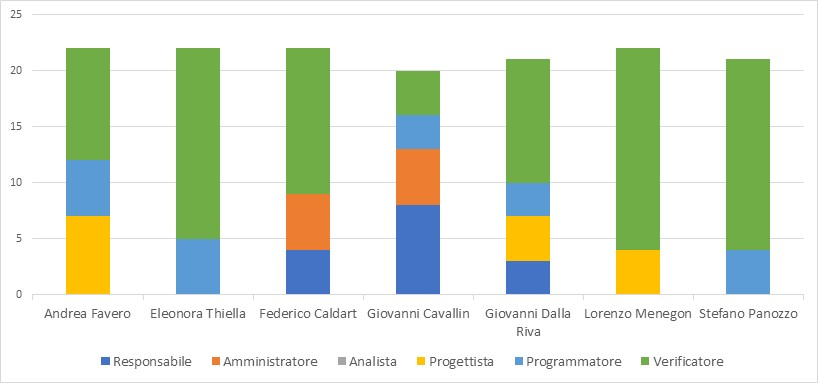
\includegraphics[scale=0.85]{img/Preventivo/Istogrammi/CodDettaglioValidazioneCollaudo.jpg}}
	\caption{Raffigurazione Prospetto Orario: Codifica in dettaglio, Validazione e Collaudo}
	\clearpage
\end{figure}
\newpage
\paragraph{Prospetto economico}
Il prospetto economico per questo periodo è illustrato in tabella. 
\begin{table}[H]
	\centerline{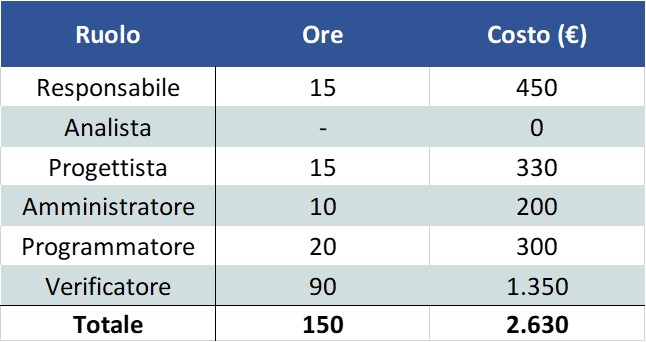
\includegraphics[scale=0.7]{img/Preventivo/CodDettaglioValidazioneCollaudoEconomico.jpg}}
	\caption{Prospetto Economico: Codifica in dettaglio, Validazione e Collaudo}
	\clearpage
\end{table}
La raffigurazione grafica del peso di ogni ruolo sul costo totale è così rappresentata: 
\begin{figure}[H]
	\centerline{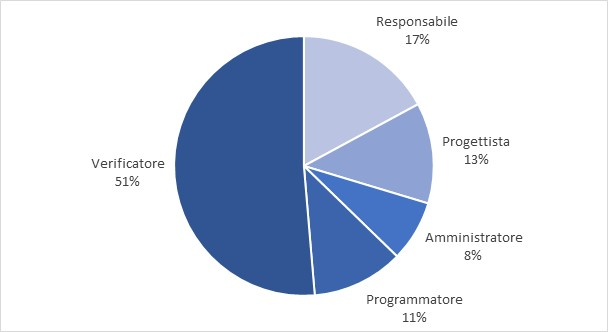
\includegraphics[scale=0.9]{img/Preventivo/Torte/CodDettaglioValidazioneCollaudo.jpg}}
	\caption{Raffigurazione Prospetto Economico: Codifica in dettaglio, Validazione e Collaudo}
	\clearpage
\end{figure} 
\newpage
\subsection{Totale}
In seguito sono presentati il prospetto orario ed economico riepilogativi per tutta la durata del progetto.\\
Si noti la differenza fra le ore totali, comprensive dell'attività di investimento iniziale a carico del gruppo, e le ore rendicontate a carico del committente.
\paragraph{Prospetto orario}
Il prospetto orario per l'intera durata del progetto è illustrato in tabella. 
\begin{table}[H]
	\centerline{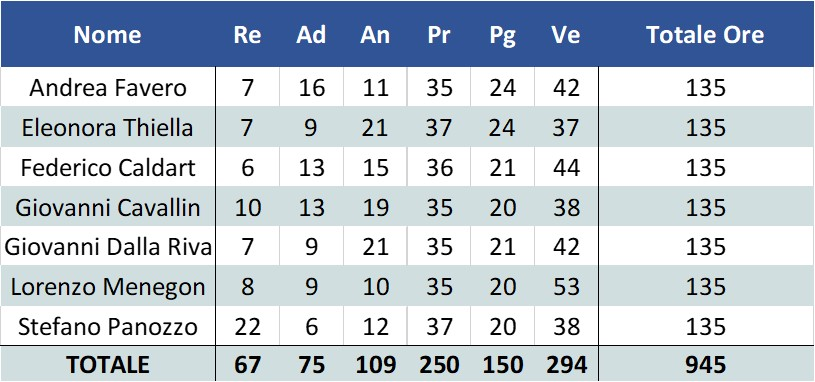
\includegraphics[scale=0.7]{img/Preventivo/TotaleOre.jpg}}
	\caption{Prospetto Orario: Riepilogo}
	\clearpage
\end{table}
La raffigurazione grafica della suddivisione dei ruoli all'interno del gruppo è così rappresentata: 
\begin{figure}[H]
	\centerline{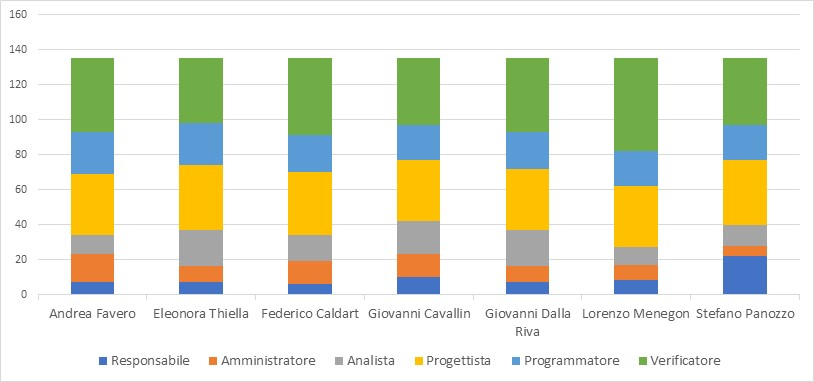
\includegraphics[scale=0.85]{img/Preventivo/Istogrammi/Totale.jpg}}
	\caption{Raffigurazione Prospetto Orario: Riepilogo ore totali}
	\clearpage
\end{figure}
\begin{figure}[H]
	\centerline{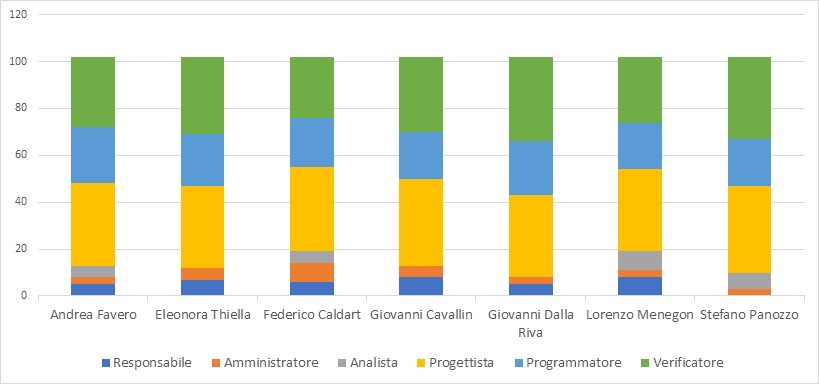
\includegraphics[scale=0.85]{img/Preventivo/Istogrammi/TotaleRendicontato.jpg}}
	\caption{Raffigurazione Prospetto Orario: Riepilogo ore totali rendicontate}
	\clearpage
\end{figure}
\paragraph{Prospetto economico}
Il prospetto economico per l'intera durata del progetto è illustrato in tabella. 
\begin{table}[H]
	\centerline{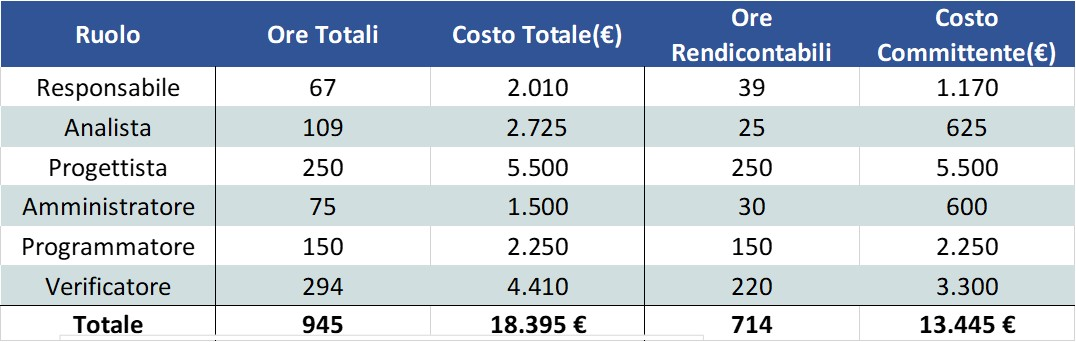
\includegraphics[scale=0.6]{img/Preventivo/TotaleEconomico.jpg}}\label{Totale}
	\caption{Prospetto Economico: Riepilogo}
	\clearpage
\end{table}
\newpage
La raffigurazione grafica del peso di ogni ruolo sul costo totale e rendicontato è così rappresentata: 
\begin{figure}[H]
	\centerline{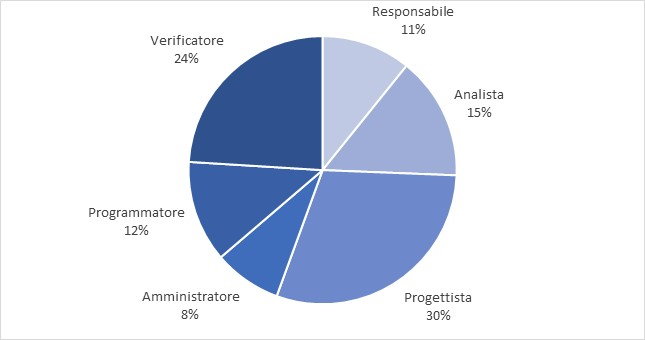
\includegraphics[scale=0.9]{img/Preventivo/Torte/Totale.jpg}}
	\caption{Raffigurazione Prospetto Economico: Riepilogo ore totali}
	\clearpage
\end{figure}
\begin{figure}[H]
	\centerline{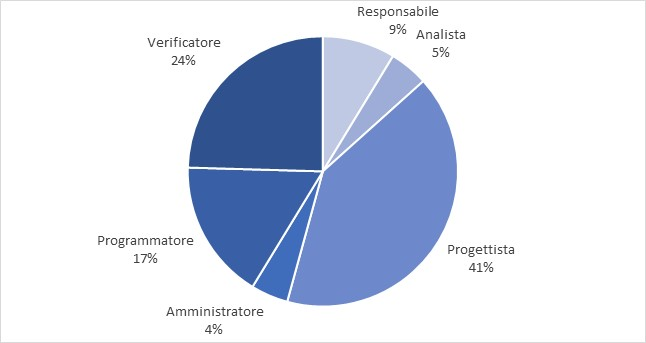
\includegraphics[scale=0.9]{img/Preventivo/Torte/TotaleRendicontato.jpg}}
	\caption{Raffigurazione Prospetto Economico: Riepilogo ore rendicontate}
	\clearpage
\end{figure}

\subsection{Conclusione}
Come si può notare nella \hyperref[Totale]{Tabella 16}, il preventivo a carico del committente per il progetto è pari a \EUR{13.445}.